\documentclass[12pt]{article}%
    \usepackage[final]{pdfpages}
    \usepackage{listings} %For code in appendix
    \usepackage{hyperref}
    \usepackage{alltt}
    \usepackage{color}
    \usepackage{sectsty}
    
    \definecolor{dkgreen}{rgb}{0,0.6,0}
    \definecolor{gray}{rgb}{0.5,0.5,0.5}
    \definecolor{mauve}{rgb}{0.58,0,0.82}
    \chapterfont{\color{blue}}
    \sectionfont{\color{cyan}}
    \lstset
    {
        frame=tb,
        language=C++,
        aboveskip=3mm,
        belowskip=3mm,
        showstringspaces=false,
        columns=flexible,
        basicstyle={\small\ttfamily},
        numbers=none,
        numberstyle=\tiny\color{gray},
        keywordstyle=\color{blue},
        commentstyle=\color{dkgreen},
        stringstyle=\color{mauve},
        breaklines=true,
        breakatwhitespace=true
        tabsize=2
    }
    \begin{document}
    \section{Usefull links for this lab}
    \begin{itemize}
        \item \url{http://www.cplusplus.com}
        \item \url{http://www.mingw.org/wiki/MinGW_for_First_Time_Users_HOWTO}
        \item \url{https://www.geeksforgeeks.org/c-data-types/}
    \end{itemize}

    \section{Lab contest}
    All given task are emplaced in automated checker system for \textbf{lab1}: \url{http://acm.kbtu.kz/cgi-bin/new-register?action=211&contest_id=125}\\
    Feel free to submit your solutions without attempt count penalty.

    \section{problem set}
    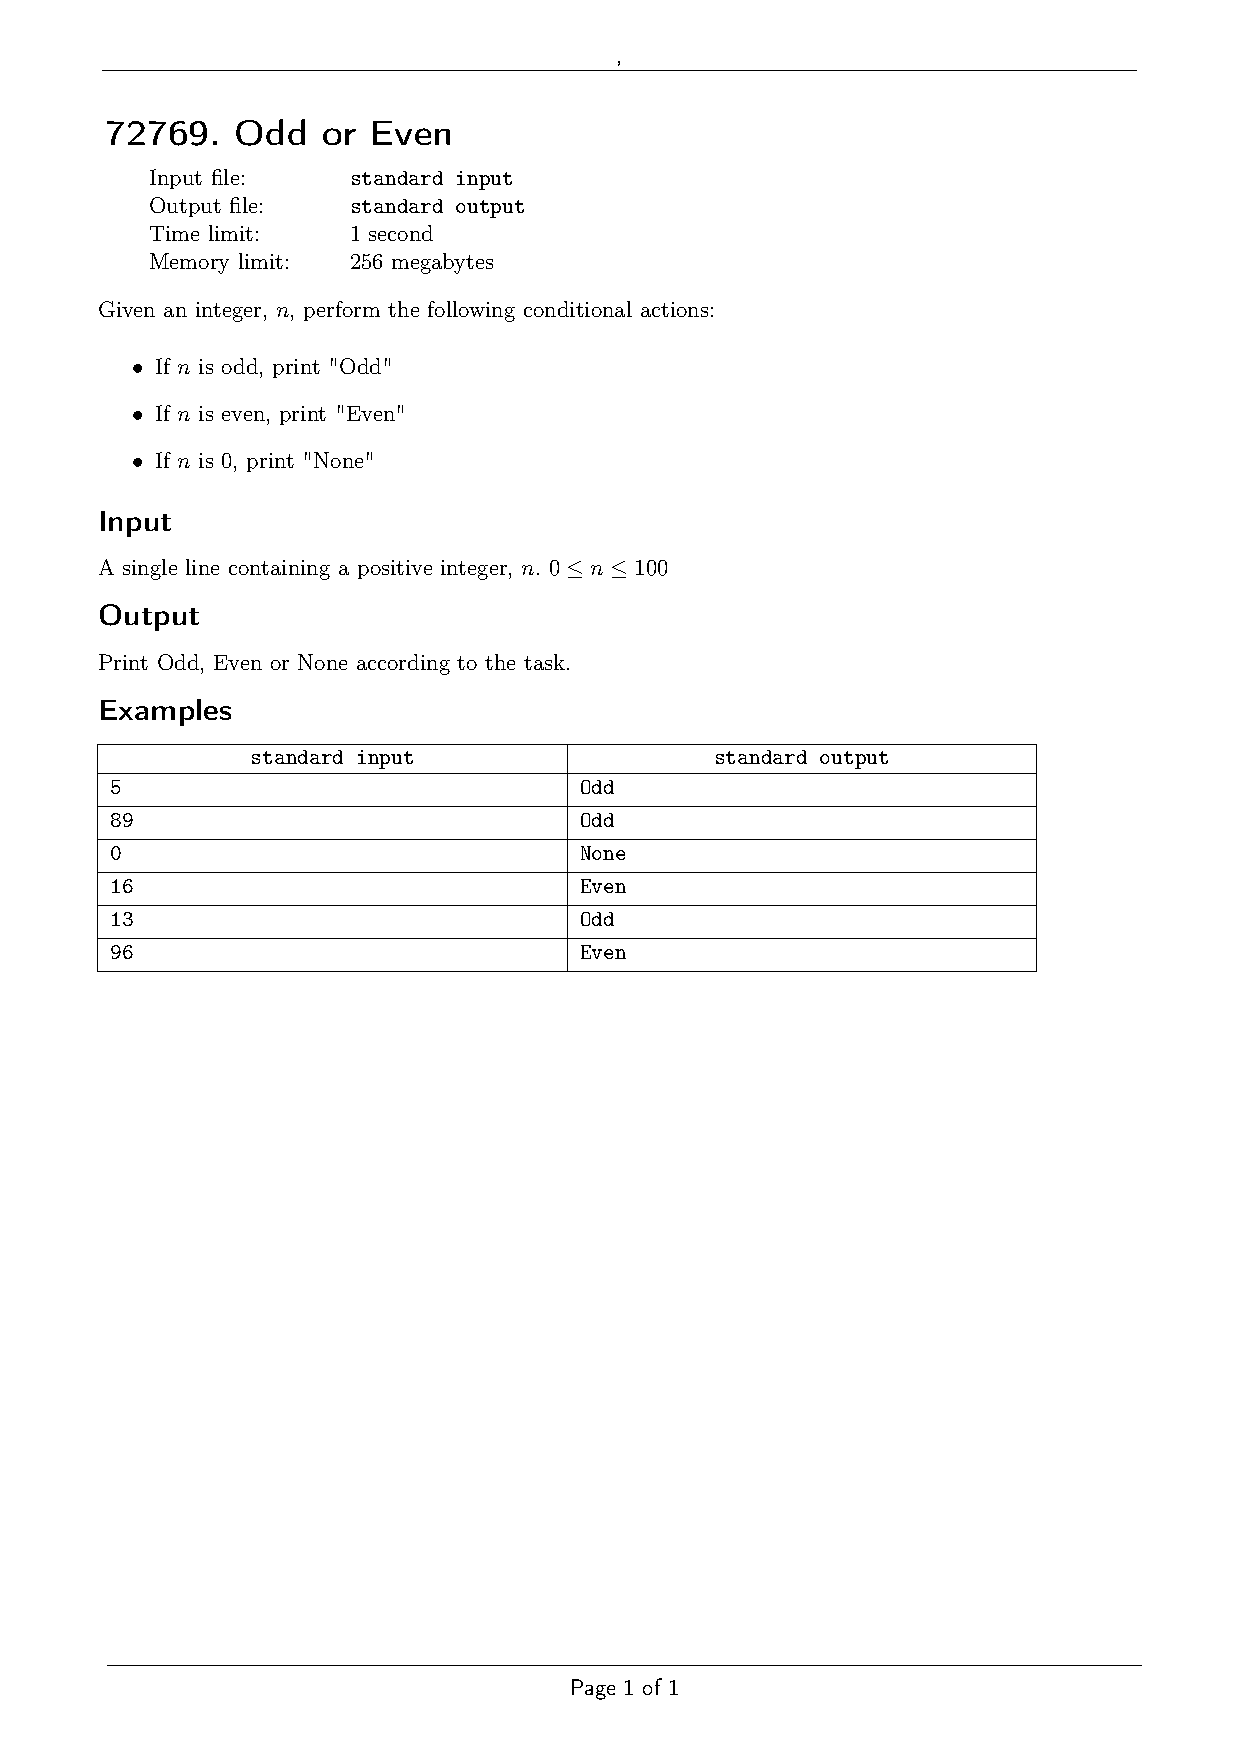
\includepdf[pages=-]{72769.pdf}

    \section{solutions}
    \textbf{problem 72769}
    \lstinputlisting{72769.cpp}

    \section{Additional tasks for this lab}
    You can solve problems starting from A to J from the link below:\\
    \url{https://informatics.msk.ru/mod/statements/view.php?id=2296}\\
    \textit{note: statements are in russian}

\end{document}